\begin{figure}[t]
\centering
\begin{minipage}{0.45\linewidth}

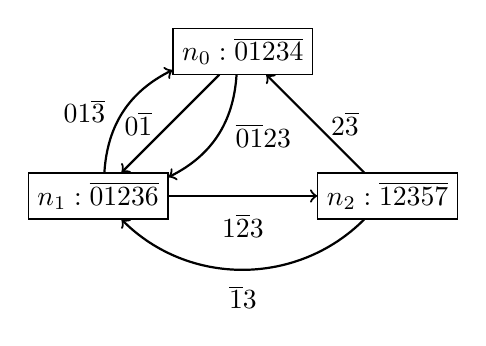
\begin{tikzpicture}[node distance = 26mm]
  \node[draw] (n0) {$n_0:\overline{01234}$};
  \node[draw,below left of=n0] (n1) {$n_1:\overline{01236}$};
  \node[draw,below right of=n0] (n2) {$n_2:\overline{12357}$};

  \draw[->,thick] (n0) -- node[left=1mm]  {$0\overline{1}$} (n1);
  \draw [->,thick] (n0) to [bend right=-30] node[right=1mm]  {$\overline{01}23$} (n1);
  \draw [->,thick] (n1) to [bend right=-30] node[left=1mm]  {$01\overline{3}$} (n0);

  \draw [->,thick] (n1) -- node[below=1mm]  {$1\overline{2}3$} (n2);
  \draw [->,thick] (n2) to [bend right=-45] node[below=2pt]  {$\overline{1}3$} (n1);

  \draw [->,thick] (n2) -- node[right=2pt]  {$2\overline{3}$} (n0);

\end{tikzpicture}
\end{minipage}
\begin{minipage}{0.50\linewidth}
  \center
\begin{tikzpicture}
\matrix [matrix of math nodes,left delimiter=(,right delimiter=),
         row sep=0.07cm,column sep=0.07cm] (m) {
\times & \times & \times &\times&\times&\times & \times & \times\\
\times & \times & \times&\times&\times&\times& 1 &\times \\
\times & \times & \times&\times&\times&1&\times &\times\\
\times & \times & \times&\times & 1 & \times &\times & \times\\
 \times & \times & \times & \times & \times & \times & \times & \times\\
 \times & \times & \times &\times & \times & \times & \times & \times\\
 \times & \times & \times & \times & \times & \times & \times & \times\\
 \times & \times & \times & \times & \times & \times&\times & \times\\};

\draw[dashed] ($0.5*(m-1-4.north east)+0.5*(m-1-5.north west)$) --
     ($0.5*(m-8-5.south east)+0.5*(m-8-4.south west)$);

\draw[dashed] ($0.5*(m-4-1.south west)+0.5*(m-5-1.north west)$) --
 ($0.5*(m-4-8.south east)+0.5*(m-5-8.north east)$);

\node[above=4pt of m-1-1] (top-1) {$M_0$};
\node[above=4pt of m-1-2] (top-2) {$M_1$};
\node[above=4pt of m-1-3] (top-3) {$M_2$};
\node[above=4pt of m-1-4] (top-4) {$M_3$};
\node[above=4pt of m-1-5] (top-5) {$M_4$};
\node[above=4pt of m-1-6] (top-6) {$M_5$};
\node[above=4pt of m-1-7] (top-7) {$M_6$};
\node[above=4pt of m-1-8] (top-8) {$M_7$};

\node[left=12pt of m-1-1] (left-1) {$M_0$};
\node[left=12pt of m-2-1] (left-2) {$M_1$};
\node[left=12pt of m-3-1] (left-3) {$M_2$};
\node[left=12pt of m-4-1] (left-4) {$M_3$};
\node[left=12pt of m-5-1] (left-5) {$M_4$};
\node[left=12pt of m-6-1] (left-6) {$M_5$};
\node[left=12pt of m-7-1] (left-7) {$M_6$};
\node[left=12pt of m-8-1] (left-8) {$M_7$};


\node[rectangle,above delimiter=\{] (del-top-1) at ($0.5*(top-1.south) +0.5*(top-4.south)$) {\tikz{\path (top-1.south west) rectangle (top-4.north east);}};
\node[above=10pt] at (del-top-1.north) {$Q-Snares$};
\node[rectangle,above delimiter=\{] (del-top-2) at ($0.5*(top-5.south) +0.5*(top-8.south)$) {\tikz{\path (top-4.south west) rectangle (top-6.north east);}};
\node[above=10pt] at (del-top-2.north) {$R-Snares$};

\node[rectangle,left delimiter=\{] (del-left-1) at ($0.5*(left-1.east) +0.5*(left-4.east)$) {\tikz{\path (left-1.north east) rectangle (left-4.south west);}};
\node[left=15pt,rotate=90,xshift=9mm] at (del-left-1.west) {$Q-Snares$};
\node[rectangle,left delimiter=\{] (del-left-2) at ($0.5*(left-5.east) +0.5*(left-8.east)$) {\tikz{\path (left-5.north east) rectangle (left-8.south west);}};
\node[left=15pt,rotate=90,xshift=9mm] at (del-left-2.west) {$R-Snares$};

% \begin{pgfonlayer}{myback}
% \foreach \element in {m-1-7,m-3-8,m-5-1,m-5-2,m-5-3,m-5-4,m-6-1,m-6-2,m-6-3,m-6-4,m-7-1,m-7-2,m-7-3,m-7-4,m-8-1,m-8-2,m-8-3,m-8-4}{
% \highlight[pink]{\element}{\element}
% }
% \foreach \element in {m-2-7,m-3-6,m-4-5}{
% \fhighlight[blue!10]{\element}{\element}
% }
% \end{pgfonlayer}

\end{tikzpicture}  
\end{minipage}


\caption{An example of VTS and corresponding pairing matrix.} \label{fig:M1}
\end{figure}

%%% Local Variables:
%%% mode: latex
%%% TeX-master: "main"
%%% End:
